\documentclass[DIN, pagenumber=false, fontsize=11pt, parskip=half]{scrartcl}
\usepackage[UTF8]{ctex}  % 中文支持
% \usepackage{ngerman}
\usepackage[utf8]{inputenc}
\usepackage[T1]{fontenc}
\usepackage{textcomp}
\usepackage{xcolor} % Required for custom red

\usepackage{geometry} % Custom margins
\usepackage{graphicx} % 插入图片需要
\usepackage{caption}  % 控制标题样式
\usepackage{tocloft} % Modifying the table of contents

% for matlab code
% bw = blackwhite - optimized for print, otherwise source is colored
\usepackage[framed,numbered,bw]{mcode}
\usepackage[most]{tcolorbox}
% for other code
%\usepackage{listings}

\setlength{\parindent}{0em}

% set section in CM
\setkomafont{section}{\normalfont\bfseries\Large}

\newcommand{\mytitle}[1]{{\noindent\Large\textbf{#1}}}
\newcommand{\mysection}[1]{\textbf{\section*{#1}}}
\newcommand{\mysubsection}[2]{\romannumeral #1) #2}

\newtcolorbox{parchmentquote}{
    enhanced,
    colback=orange!5!white,   % 浅米黄色背景
    colframe=orange!50!black,
    boxrule=0.5pt,
    arc=2pt,                  % 细微圆角
    boxsep=5pt,
    before skip=10pt,
    after skip=10pt,
    fontupper=\itshape,
    borderline west={2pt}{0pt}{orange!80!black} % 加厚的左装饰线
}
%===================================
\begin{document}

\noindent\textbf{课下练习} \hfill \textbf{online course}\\
primary school \hfill Liu\\

\mytitle{运算律与几何综合应用 \hfill \today}
\newline
\begin{parchmentquote}
    复习长方形、正方形、平行四边形、三角形、梯形和圆的面积公式。\newline

\end{parchmentquote}


%===================================
\section{几何图形面积}
\begin{enumerate}
    \item 一个长方形的长是 $2.5$ 厘米，宽是长的 $\frac{2}{5}$，求它的面积。
    \item 一个正方形的边长是 $3.2$ 厘米，求它的面积。
    \item 一个平行四边形的底是 $4$ 厘米，高是底的 $1.2$ 倍，求它的面积。
    \item 一个三角形的底是 $6$ 厘米，高是底的 $\frac{1}{2}$，求它的面积。
    \item 一个梯形的上底是 $3$ 厘米，下底是上底的 $2$ 倍，高是 $4$ 厘米，求它的面积。
    \item 一个圆的半径是 $2$ 厘米，求它的面积。
\end{enumerate}

\section{综合应用}

\subsection{年龄差}
甲对乙说：“我在你这个年龄时，你才 3 岁。”
乙对甲说：“我到你这个年龄时，你就 24 岁了。”
求甲、乙现在各多少岁？
\subsection{面积差}
1. 已知正方形的边长是 $8$ 厘米，CE=$10cm$。$\triangle ECG$比$\triangle ADF$大多少平方厘米？（如图.1）\newline
2. 已知ABCD是一个平行四边形，角BCE是一个直角，CG=$6cm$，EF=$4cm$。已知阴影部分面积比$\triangle EFG$大$10cm^2$，求BC的长度。（如图.2）



\begin{figure}[htbp]
    % 左边图片
    \begin{minipage}{0.45\textwidth}
        \centering
        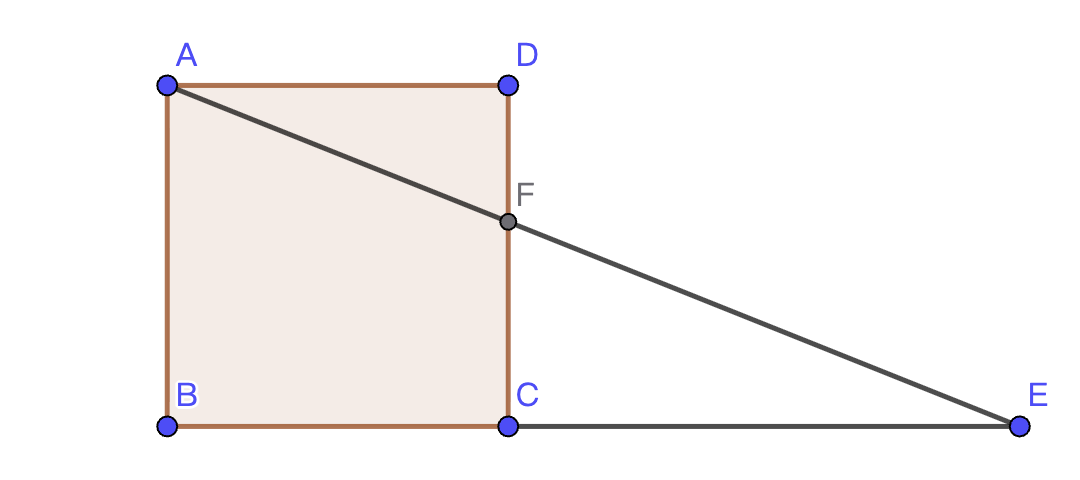
\includegraphics[width=\textwidth]{square_1.png}
        \caption{图1：2-1图片}
    \end{minipage}
    \hfill
    % 右边图片
    \begin{minipage}{0.45\textwidth}
        \centering
        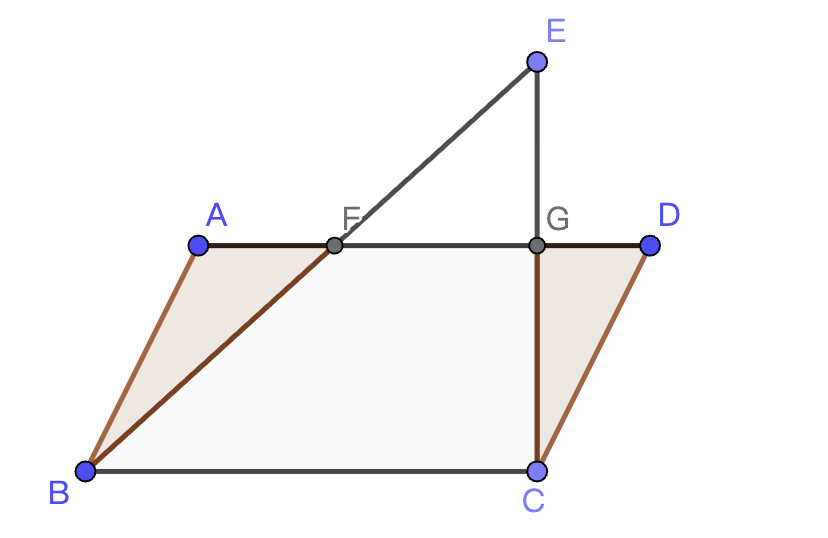
\includegraphics[width=\textwidth]{square_2.png}
        \caption{图2：右边的图片}
    \end{minipage}
\end{figure}
\subsection{列方程}
这里解方程有点难度，本身的知识点不难\newline 
\begin{enumerate}
    \item 已知一个长方形的长是宽的 $2$ 倍，面积是 $72$ 平方厘米，求长和宽的长度。
    \item 已知一个三角形的底是高的 $3$ 倍，面积是 $13.5$ 平方厘米，求底和高的长度。
\end{enumerate}

\end{document}